\documentclass[PI,LAB]{HSEUniversity}
% Возможные опции: KR или VKR; PI или BI
\usepackage{svg}
\usepackage{listings}

\title{Организация паттернов проектирования. Порождающий паттерн Строитель}
\author{Виноградов Никита Андреевич}
\supervisor{к.т.н., доцент кафедры Информационных технологий в бизнесе НИУ ВШЭ-Пермь}{А.В.~Кычкин}

\Year{2020}


% Ссылка на файл с описание библиографии
\bibliography{library.bib}

%%%%%%%%%%%%%%%%%%%%%%%%%%%%%%%%
%%% ТЕКСТ РАБОТЫ %%%%%%%%%%%%%%%
\begin{document}

    % Обязательные элементы оформления: заголовочный слайд, аннотация, оглавление
    \maketitle



    \chapter{Строитель}
      Порождающий паттерн проектирования, который позволяет создавать сложные объекты пошагово. 
    \section{Назначение}
   Строитель даёт возможность использовать один и тот же код строительства для получения разных представлений объектов
    \section{Структура}

    \begin{FIGURE}[h]{Структура классов паттерна строитель\label{fig:example-figure}}
       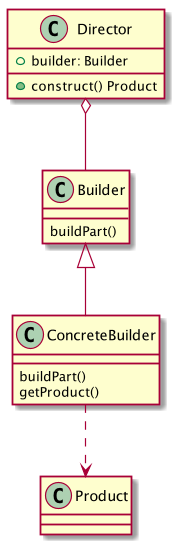
\includegraphics[width=0.2\textwidth]{../out/diagrams/builder/builder_default_class}
    \end{FIGURE}

    \textbf{Участники:}
   		\begin{itemize}
   			\item \emph{Director} - класс который вызывает методы строителя
   			\item \emph{Builder} - интерфейс задает базу для сборки продукта
   			\item \emph{ConcreteBuilder} - класc который делает сборку продукта из частей
   			\item \emph{Product} - класс для которого задаются параметры
   		\end{itemize}

 \begin{FIGURE}[h]{Диаграмма последовательности паттерна строитель\label{fig:example-figure}}
	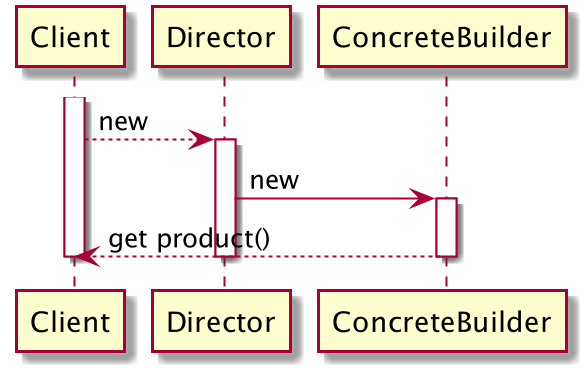
\includegraphics[width=0.5\textwidth]{../out/diagrams/builder/builder_default_sq}
\end{FIGURE}
    \section{Способ применения}
    Данный паттерн применим когда в коде программы встречается конструктор с большим количеством параметров которые позволяют разделить части конструктора на блоки.
    
    \chapter{Реализация паттернов}

    \section{Диаграмма классов}
     \begin{FIGURE}[h]{Диаграмма классов паттерна строитель\label{fig:example-figure}}
    	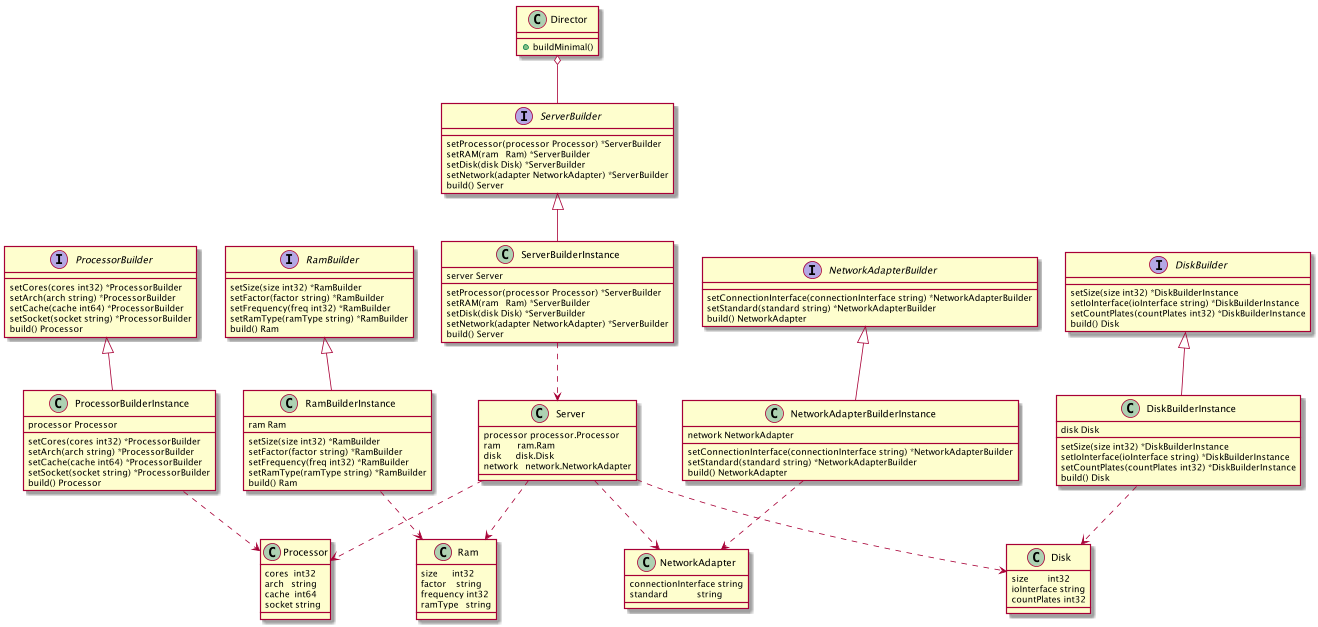
\includegraphics[width=\textwidth]{../out/diagrams/builder/builder-class}
    \end{FIGURE}
	\emph{Участники:}
	\begin{itemize}
		\item \emph{Server, Processor, Ram,Disk, Network} - класссы для которых необходимо задавать параметры
		\item \emph{ProcessorBuilder, RamBuilder, ServerBuilder, NetworkAdapterBuilder, DiskBuilder} - классы строителей которые задают параметры для объекта и делают сборку продукта
		\item \emph{Director} - класс который задает запросы на создание объектов
	\end{itemize}
\pagebreak
    \section{Диаграмма последовательности }
  
	\begin{FIGURE}[h]{Диаграмма классов паттерна строитель\label{fig:example-figure}}
		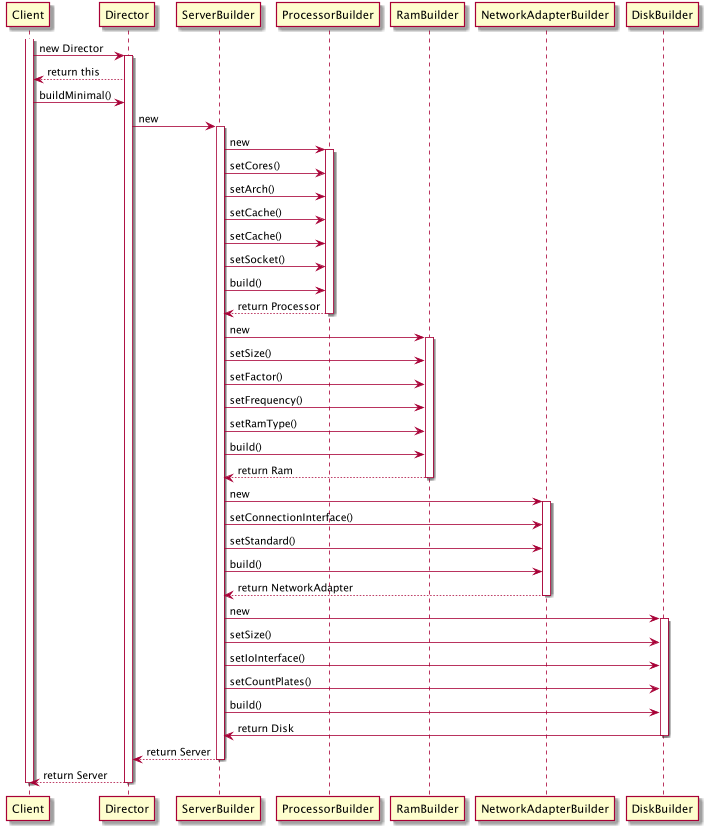
\includegraphics[width=0.9\textwidth]{../out/diagrams/builder/builder_seq}
	\end{FIGURE}
	\emph{Участники:}
\begin{itemize}
	\item \emph{Server,Processor,Ram,Disk,Network} - класссы для которых необходимо задавать параметры
	\item \emph{ProcessorBuilder, RamBuilder, ServerBuilder, NetworkAdapterBuilder, DiskBuilder} - классы строителей которые задают параметры для объекта и делают сборку продукта
	\item \emph{Director} - класс который задает запросы на создание объектов
\end{itemize}
   


    \section{Код программы}
    \lstset{extendedchars=\true}
    \begin{lstlisting}[language=Go]
    package server
    
    import (
    "fmt"
    "hse.pattern/lab2.Builder/code/disk"
    "hse.pattern/lab2.Builder/code/network"
    "hse.pattern/lab2.Builder/code/processor"
    "hse.pattern/lab2.Builder/code/ram"
    )
    
    type PerformanceMonitor interface {
    getPerformance() float32
    info() string
    }
    
    type Server struct {
    processor *processor.Processor
    ram       *ram.Ram
    disk      *disk.Disk
    network   *network.NetworkAdapter
    }
    
    type ServerBuilder interface {
    setProcessor(processor processor.Processor) *ServerBuilder
    setRAM(ram ram.Ram) *ServerBuilder
    setDisk(disk disk.Disk) *ServerBuilder
    setNetwork(adapter network.NetworkAdapter) *ServerBuilder
    build() Server
    }
    
    type ServerIstanceBuilder struct {
    server *Server
    }
    
    func NewServerIstanceBuilder() *ServerIstanceBuilder {
    return &ServerIstanceBuilder{server: &Server{}}
    }
    
    func (s ServerIstanceBuilder) setProcessor(processor processor.Processor) *ServerIstanceBuilder {
    s.server.processor = &processor
    return &s
    }
    
    func (s ServerIstanceBuilder) setRAM(ram ram.Ram) *ServerIstanceBuilder {
    s.server.ram = &ram
    return &s
    }
    
    func (s ServerIstanceBuilder) setDisk(disk disk.Disk) *ServerIstanceBuilder {
    s.server.disk = &disk
    return &s
    }
    
    func (s ServerIstanceBuilder) setNetwork(adapter network.NetworkAdapter) *ServerIstanceBuilder {
    s.server.network = &adapter
    return &s
    }
    func (s ServerIstanceBuilder) build() Server {
    fmt.Println("flex")
    return *s.server
    }
    
    func GenerateServer() Server {
    sBuilder := NewServerIstanceBuilder()
    fmt.Println("flex")
    ss := sBuilder.setDisk(disk.GenerateDisk()).setProcessor(processor.GenerateProcessor()).setNetwork(network.GenerateNetwork()).setRAM(ram.GenerateRam()).build()
    fmt.Println(ss.processor)
    return ss
    }
    
    \end{lstlisting}

\end{document}
